\documentclass[a4paper]{tufte-handout}
% Shared preamble for all lab reports (Tufte handout layout).
%
% Usage, from labN/report/labN_report.tex:
%   \documentclass[a4paper,justified]{tufte-handout}
%   % Shared preamble for all lab reports (Tufte handout layout).
%
% Usage, from labN/report/labN_report.tex:
%   \documentclass[a4paper,justified]{tufte-handout}
%   % Shared preamble for all lab reports (Tufte handout layout).
%
% Usage, from labN/report/labN_report.tex:
%   \documentclass[a4paper,justified]{tufte-handout}
%   \input{../../report-style/preamble}
%   \labtitle{2}{ROS, TF and Quaternions}
%
% Build: latexmk -pdf labN_report.tex

\usepackage{amsmath,amssymb,bm}
\usepackage{booktabs,tabularx,array}
\usepackage{graphicx}
\usepackage{xcolor}
\usepackage{textcomp}
\usepackage{listings}
\usepackage[most]{tcolorbox}
\usepackage{siunitx}
\usepackage{cleveref}

\setcounter{secnumdepth}{2}
\crefname{section}{Section}{Sections}
\crefname{figure}{Figure}{Figures}
\crefname{table}{Table}{Tables}
\crefname{listing}{Listing}{Listings}
% In main-column table/figure floats a \label after \caption refers to the
% section (tufte-latex with the current kernel); write
% \caption{Text.\protect\label{key}} instead. Margin floats are unaffected.
\hypersetup{colorlinks=true, allcolors=[rgb]{0.12,0.25,0.55}}

% --- Author and course -------------------------------------------------------
\newcommand{\studentname}{Xuanye Xu}
\newcommand{\studentids}{24020036071 / H00490299}
\newcommand{\coursename}{Robotics Integration I --- VNAV Labs}

% \labtitle{<lab number>}{<topic>}
\newcommand{\labtitle}[2]{%
  \title[Lab #1: #2]{Lab #1 Report: #2}%
  \author[\studentname]{\studentname\\[2pt]
    {\normalsize\normalfont Student ID \studentids\\ \coursename}}%
  \date{\today}}

% --- Grading items -----------------------------------------------------------
% \gradeditem{<label>}{<title>}{<points>} starts a section for one grading item.
\newcommand{\gradeditem}[3]{%
  \section{#2\texorpdfstring{\enspace{\normalfont\small[#3~pts]}}{ [#3 pts]}}\label{#1}}

% Evidence summary shown at the end of each graded section.
\newtcolorbox{evidence}{enhanced, breakable, frame hidden, arc=0pt,
  colback=black!4, borderline west={1.2pt}{0pt}{black!55},
  left=6pt, right=4pt, top=3pt, bottom=3pt,
  before upper={\textsc{Evidence}\quad}}

% Marks unfinished content in red; a final report must contain none.
\newcommand{\pending}[1]{\textcolor{red}{[PENDING: #1]}}

% --- Code and terminal output ------------------------------------------------
\lstdefinestyle{code}{language=C++, basicstyle=\ttfamily\footnotesize,
  keywordstyle=\bfseries, commentstyle=\itshape\color{black!60},
  numbers=left, numberstyle=\tiny\color{black!50}, xleftmargin=1.5em,
  columns=fullflexible, keepspaces, breaklines, showstringspaces=false,
  upquote=true}
\lstdefinestyle{log}{basicstyle=\ttfamily\scriptsize, frame=leftline,
  framerule=0.6pt, rulecolor=\color{black!40}, xleftmargin=0.8em,
  columns=fullflexible, keepspaces, breaklines, upquote=true}
\lstset{style=log}

%   \labtitle{2}{ROS, TF and Quaternions}
%
% Build: latexmk -pdf labN_report.tex

\usepackage{amsmath,amssymb,bm}
\usepackage{booktabs,tabularx,array}
\usepackage{graphicx}
\usepackage{xcolor}
\usepackage{textcomp}
\usepackage{listings}
\usepackage[most]{tcolorbox}
\usepackage{siunitx}
\usepackage{cleveref}

\setcounter{secnumdepth}{2}
\crefname{section}{Section}{Sections}
\crefname{figure}{Figure}{Figures}
\crefname{table}{Table}{Tables}
\crefname{listing}{Listing}{Listings}
% In main-column table/figure floats a \label after \caption refers to the
% section (tufte-latex with the current kernel); write
% \caption{Text.\protect\label{key}} instead. Margin floats are unaffected.
\hypersetup{colorlinks=true, allcolors=[rgb]{0.12,0.25,0.55}}

% --- Author and course -------------------------------------------------------
\newcommand{\studentname}{Xuanye Xu}
\newcommand{\studentids}{24020036071 / H00490299}
\newcommand{\coursename}{Robotics Integration I --- VNAV Labs}

% \labtitle{<lab number>}{<topic>}
\newcommand{\labtitle}[2]{%
  \title[Lab #1: #2]{Lab #1 Report: #2}%
  \author[\studentname]{\studentname\\[2pt]
    {\normalsize\normalfont Student ID \studentids\\ \coursename}}%
  \date{\today}}

% --- Grading items -----------------------------------------------------------
% \gradeditem{<label>}{<title>}{<points>} starts a section for one grading item.
\newcommand{\gradeditem}[3]{%
  \section{#2\texorpdfstring{\enspace{\normalfont\small[#3~pts]}}{ [#3 pts]}}\label{#1}}

% Evidence summary shown at the end of each graded section.
\newtcolorbox{evidence}{enhanced, breakable, frame hidden, arc=0pt,
  colback=black!4, borderline west={1.2pt}{0pt}{black!55},
  left=6pt, right=4pt, top=3pt, bottom=3pt,
  before upper={\textsc{Evidence}\quad}}

% Marks unfinished content in red; a final report must contain none.
\newcommand{\pending}[1]{\textcolor{red}{[PENDING: #1]}}

% --- Code and terminal output ------------------------------------------------
\lstdefinestyle{code}{language=C++, basicstyle=\ttfamily\footnotesize,
  keywordstyle=\bfseries, commentstyle=\itshape\color{black!60},
  numbers=left, numberstyle=\tiny\color{black!50}, xleftmargin=1.5em,
  columns=fullflexible, keepspaces, breaklines, showstringspaces=false,
  upquote=true}
\lstdefinestyle{log}{basicstyle=\ttfamily\scriptsize, frame=leftline,
  framerule=0.6pt, rulecolor=\color{black!40}, xleftmargin=0.8em,
  columns=fullflexible, keepspaces, breaklines, upquote=true}
\lstset{style=log}

%   \labtitle{2}{ROS, TF and Quaternions}
%
% Build: latexmk -pdf labN_report.tex

\usepackage{amsmath,amssymb,bm}
\usepackage{booktabs,tabularx,array}
\usepackage{graphicx}
\usepackage{xcolor}
\usepackage{textcomp}
\usepackage{listings}
\usepackage[most]{tcolorbox}
\usepackage{siunitx}
\usepackage{cleveref}

\setcounter{secnumdepth}{2}
\crefname{section}{Section}{Sections}
\crefname{figure}{Figure}{Figures}
\crefname{table}{Table}{Tables}
\crefname{listing}{Listing}{Listings}
% In main-column table/figure floats a \label after \caption refers to the
% section (tufte-latex with the current kernel); write
% \caption{Text.\protect\label{key}} instead. Margin floats are unaffected.
\hypersetup{colorlinks=true, allcolors=[rgb]{0.12,0.25,0.55}}

% --- Author and course -------------------------------------------------------
\newcommand{\studentname}{Xuanye Xu}
\newcommand{\studentids}{24020036071 / H00490299}
\newcommand{\coursename}{Robotics Integration I --- VNAV Labs}

% \labtitle{<lab number>}{<topic>}
\newcommand{\labtitle}[2]{%
  \title[Lab #1: #2]{Lab #1 Report: #2}%
  \author[\studentname]{\studentname\\[2pt]
    {\normalsize\normalfont Student ID \studentids\\ \coursename}}%
  \date{\today}}

% --- Grading items -----------------------------------------------------------
% \gradeditem{<label>}{<title>}{<points>} starts a section for one grading item.
\newcommand{\gradeditem}[3]{%
  \section{#2\texorpdfstring{\enspace{\normalfont\small[#3~pts]}}{ [#3 pts]}}\label{#1}}

% Evidence summary shown at the end of each graded section.
\newtcolorbox{evidence}{enhanced, breakable, frame hidden, arc=0pt,
  colback=black!4, borderline west={1.2pt}{0pt}{black!55},
  left=6pt, right=4pt, top=3pt, bottom=3pt,
  before upper={\textsc{Evidence}\quad}}

% Marks unfinished content in red; a final report must contain none.
\newcommand{\pending}[1]{\textcolor{red}{[PENDING: #1]}}

% --- Code and terminal output ------------------------------------------------
\lstdefinestyle{code}{language=C++, basicstyle=\ttfamily\footnotesize,
  keywordstyle=\bfseries, commentstyle=\itshape\color{black!60},
  numbers=left, numberstyle=\tiny\color{black!50}, xleftmargin=1.5em,
  columns=fullflexible, keepspaces, breaklines, showstringspaces=false,
  upquote=true}
\lstdefinestyle{log}{basicstyle=\ttfamily\scriptsize, frame=leftline,
  framerule=0.6pt, rulecolor=\color{black!40}, xleftmargin=0.8em,
  columns=fullflexible, keepspaces, breaklines, upquote=true}
\lstset{style=log}

\labtitle{2}{ROS, TF and Quaternions}

\begin{document}
\maketitle

\begin{abstract}
ROS~1 Noetic was installed in Ubuntu~20.04 under WSL~2 and verified with
turtlesim.
In the two-drone scenario, AV1 flies a circle and AV2 an arc of a parabola;
their poses were published as \texttt{tf2} transforms, and the relative
transform was looked up to plot three trajectories in RViz.
Seen from AV1, AV2 moves on an ellipse in the plane $z - 2y = 1$ with
semi-axes $\tfrac12$ and $\tfrac{\sqrt5}{2}$; this was derived with
homogeneous transforms and confirmed on 300 tf samples to round-off level.
Three properties of the quaternion multiplication matrices were proved.
\end{abstract}

\section*{Grading Map}

\begin{table*}[h]
\small
\begin{tabularx}{\linewidth}{@{}l r l X@{}}
\toprule
Grading item & Points & Section & Evidence \\
\midrule
ROS installation & 20 & \cref{sec:install} & Environment table, turtlesim screenshot, node and topic listing \\
Two-drone motion & 40 & \cref{sec:drones} & Answers on nodes, topics and the launch file; publisher code; static and dynamic scenes; TF tree; \texttt{/tf} rate \\
Trajectories & 30 & \cref{sec:traj} & Three trajectories in the \texttt{world} and \texttt{av1} frames; numerical check against the analytic model \\
Mathematical derivation & 10 & \cref{sec:math} & Five derivations with homogeneous transforms \\
Quaternion properties & 10 & \cref{sec:quat} & Three proofs; note on a sign difference in the lecture slides \\
\bottomrule
\end{tabularx}
\end{table*}

\section{Lab Introduction}\label{sec:intro}
This lab introduces the Robot Operating System (ROS~1 Noetic) and the \texttt{tf2}
transform library.
Two simulated drones are driven by publishing their poses as time-varying
transforms, their trajectories are drawn in RViz in different reference frames,
and the observed relative motion is explained with homogeneous transforms.
The last part proves several properties of the quaternion multiplication
matrices.
The tasks follow the MIT VNAV 2023 Lab~2 exercises,\cite{vnav2023lab2} using the
ROS~1 template code from the \texttt{VNAV2023} release.\cite{vnavlabs}
The working environment is summarised in \cref{tab:env}.

\gradeditem{sec:install}{ROS Installation}{20}

\paragraph{Platform.}
All ROS work runs in Ubuntu~20.04 under WSL~2 on an x86-64 Windows~11 desktop
(\cref{tab:env}).
Commands are issued from a MacBook over SSH; the Windows desktop is viewed with
Moonlight, and Linux GUI programs (turtlesim, RViz) are displayed on it through
WSLg.
\marginnote{Apple-silicon Macs cannot run the x86-64 simulators required in
Labs~3 and~4, so the whole course uses this x86-64 host.}

\begin{table}[h]
\small
\begin{tabularx}{\linewidth}{@{}l X@{}}
\toprule
Component & Version \\
\midrule
Windows host & 10.0.26200 (Windows 11), WSL 2.7.12, WSLg 1.0.73 \\
Linux & Ubuntu 20.04.6 LTS, kernel 6.18.33.2-microsoft-standard-WSL2, x86\_64 \\
ROS & Noetic (\texttt{ros-noetic-desktop-full} 1.5.0) \\
Key packages & roscpp 1.17.4, tf2\_ros 0.7.10, rviz 1.14.26, turtlesim 0.10.3 \\
Build tools & catkin\_tools 0.9.4, g++ 9.4.0, CMake 3.16.3 \\
Lab code & VNAV-labs tag \texttt{VNAV2023}, commit \texttt{7d234d8} \\
\bottomrule
\end{tabularx}
\caption{Software environment, taken from \texttt{results/logs/environment.txt}.\protect\label{tab:env}}
\end{table}

\paragraph{Installation.}
The ROS key used by older installation guides expired on 1~June~2025, so the
package source was configured with the official \texttt{ros-apt-source}
package (version 1.3.0), which installs the current signing key and the
\texttt{packages.ros.org} source.\cite{roskeymigration}
The desktop-full metapackage and the build tools were then installed with
\texttt{apt}: 1487 new packages, including 234 \texttt{ros-noetic-*} packages,
with no apt errors or warnings.
Finally \texttt{rosdep} was initialised and updated with
\texttt{--include-eol-distros}, because Noetic reached end of life in May~2025,
and \texttt{source /opt/ros/noetic/setup.bash} was added to \texttt{\textasciitilde/.bashrc}.
\marginnote{Full command list and apt summary:
\texttt{results/logs/ros\_install\_summary.txt}.}

\paragraph{Turtlesim test.}
\texttt{roscore}, \texttt{turtlesim\_node} and \texttt{turtle\_teleop\_key}
were started in three shells.
The teleoperation node reads the arrow keys and publishes
\texttt{geometry\_msgs/Twist} messages on \texttt{/turtle1/cmd\_vel}, which the
simulator subscribes to (\cref{lst:turtle}).
While the turtle was driven by hand, all 32 published commands were recorded:
12 forward and 2 backward ($v_x=\pm 2$), 7 left and 11 right turns
($\omega_z=\pm 2$).
\Cref{fig:turtle} shows the resulting path.

\begin{marginfigure}
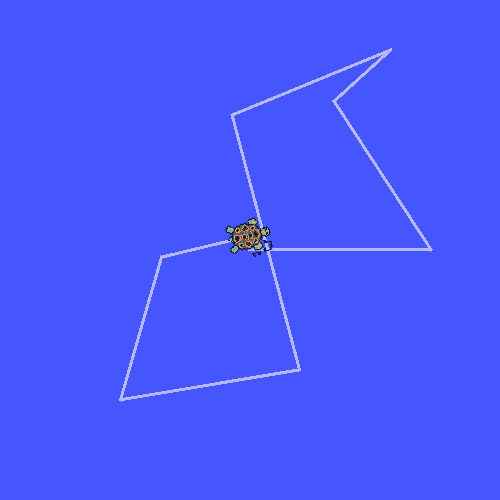
\includegraphics[width=\linewidth]{../results/screenshots/turtlesim_teleop.png}
\caption{Turtlesim window after keyboard teleoperation; the trail is the path
driven with the arrow keys.}
\label{fig:turtle}
\end{marginfigure}

\lstinputlisting[linerange={2-5,12-19}, caption={Nodes and the command topic
during teleoperation (\texttt{results/logs/turtlesim\_nodes\_topics.txt}).},
label=lst:turtle]{../results/logs/turtlesim_nodes_topics.txt}

\begin{evidence}
\cref{tab:env} (versions); \texttt{ros\_install\_summary.txt} (installation);
\cref{fig:turtle} (turtlesim with keyboard-driven path); \cref{lst:turtle}
(nodes and topic connections); \texttt{turtle\_cmd\_vel.csv} (32 recorded
keyboard commands).
\end{evidence}

\gradeditem{sec:drones}{ROS Basics and Two-Drone Motion}{40}

The package \texttt{two\_drones\_pkg} was taken unchanged from the
\texttt{VNAV2023} release\cite{vnavlabs} and built with \texttt{catkin build}
in \texttt{\textasciitilde/vnav\_ws}.
Before the first build one defect of the template was fixed
(\cref{lst:order}): \texttt{plots\_publisher\_node} declared its
\texttt{tf\_listener} before the \texttt{tf\_buffer} it is constructed from.
C++ constructs members in declaration order, so the listener received a
reference to a buffer that did not exist yet; reordering the declarations
removes this undefined behaviour.
The loop that waits for the first transforms also received a
\SI{0.1}{s} sleep so that it no longer spins at full CPU.
All builds finished without compiler warnings.

\lstinputlisting[style=code, linerange={14-17}, firstnumber=14,
caption={Member declarations in \texttt{plots\_publisher\_node.cpp} after the fix.},
label=lst:order]{../two_drones_pkg/src/plots_publisher_node.cpp}

\subsection{Nodes, topics and the launch file}

The static scenario was started with
\texttt{roslaunch two\_drones\_pkg two\_drones.launch static:=True}
(\cref{fig:static}); all answers below were checked on the running system.
\marginnote{Raw output: \texttt{results/logs/static\_nodes\_topics.txt},
\texttt{manual\_static\_run.txt}, \texttt{nonstatic\_template\_run.txt}.}

\paragraph{Q1: running nodes.}
Apart from \texttt{/rosout}, which belongs to \texttt{roscore}, four nodes run:
\texttt{/av1broadcaster} and \texttt{/av2broadcaster}
(both \texttt{tf2\_ros/static\_transform\_publisher}),
\texttt{/plots\_publisher\_node} and \texttt{/rviz}.

\paragraph{Q2: the same scenario without roslaunch.}
Each command of \cref{lst:manual} runs in its own terminal after sourcing the
workspace.
The \texttt{\_\_name:=} remappings give the nodes the names used in the launch
file; without the last one RViz registers under an anonymous name such as
\texttt{/rviz\_1790321167892688005}.
With these commands the node list and the \texttt{/tf\_static} connections
were identical to the launch-file run, and RViz showed the same scene.

\lstinputlisting[linerange={3-7}, caption={Commands that reproduce the static
scenario, one per terminal.}, label=lst:manual]{../results/logs/manual_static_run.txt}

\paragraph{Q3: topics.}
\Cref{tab:pubsub} lists the connections reported by \texttt{rosnode info}.
The frames \texttt{av1} and \texttt{av2} are published by
\texttt{/av1broadcaster} and \texttt{/av2broadcaster} on \texttt{/tf\_static}.
The drone meshes come from the \texttt{visualization\_msgs/MarkerArray} on
\texttt{/visuals}, published by \texttt{/plots\_publisher\_node}: unticking the
MarkerArray display removes both meshes while the TF axes stay
(\cref{fig:markeroff}).

\begin{table}[h]
\small
\begin{tabularx}{\linewidth}{@{}l X X@{}}
\toprule
Node & Publishes & Subscribes \\
\midrule
\texttt{/av1broadcaster} & \texttt{/tf\_static} & --- \\
\texttt{/av2broadcaster} & \texttt{/tf\_static} & --- \\
\texttt{/plots\_publisher\_node} & \texttt{/visuals} & \texttt{/tf}, \texttt{/tf\_static} \\
\texttt{/rviz} & \texttt{/clicked\_point}, \texttt{/initialpose}, \texttt{/move\_base\_simple/goal} & \texttt{/tf}, \texttt{/tf\_static}, \texttt{/visuals} \\
\bottomrule
\end{tabularx}
\caption{Topics of the static scenario, \texttt{/rosout} omitted. The three
topics published by RViz belong to its interactive tools and have no
subscribers here.\protect\label{tab:pubsub}}
\end{table}

\begin{marginfigure}
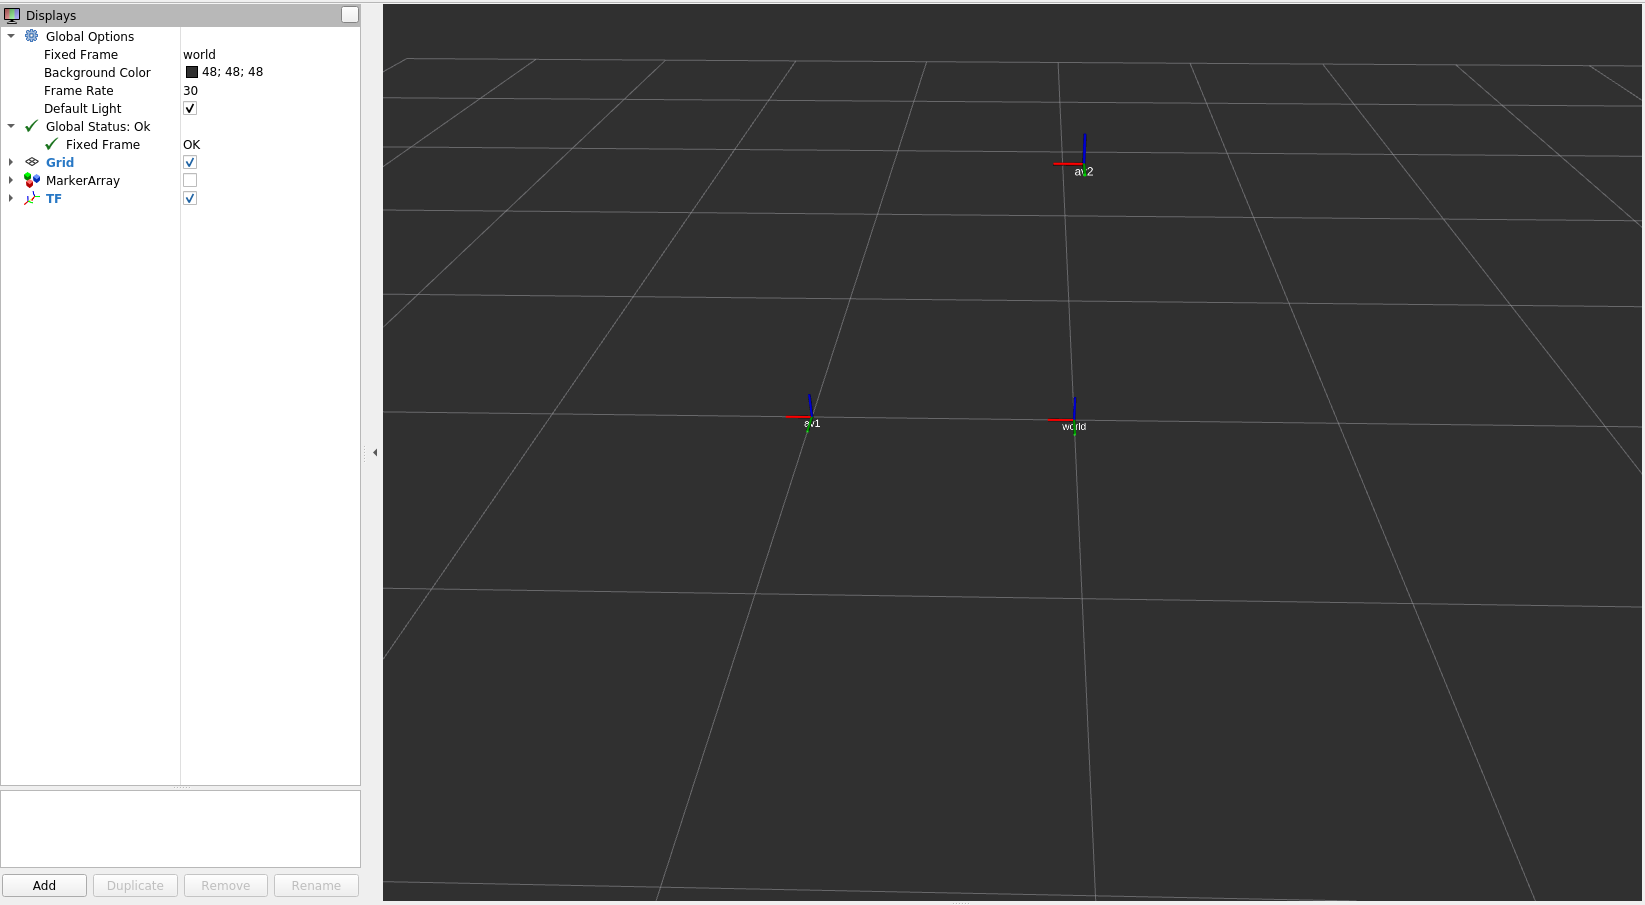
\includegraphics[width=\linewidth]{../results/screenshots/static_markerarray_off.png}
\caption{Static scene with the MarkerArray display unticked: the meshes
disappear, the TF axes of \texttt{world}, \texttt{av1} and \texttt{av2} remain.}
\label{fig:markeroff}
\end{marginfigure}

\paragraph{Q4: omitting \texttt{static:=True}.}
The launch file declares \texttt{<arg name="static" default="false"/>}.
The two static publishers sit in \texttt{<group if="\$(arg static)">} and are
started only when the argument is true, while
\texttt{frames\_publisher\_node} carries \texttt{unless="\$(arg static)"} and
is started only when it is false.
Without the argument the launch therefore replaces the fixed transforms by
the time-varying ones of \texttt{frames\_publisher\_node}.
With the unmodified template this node publishes nothing, which was observed
directly (\cref{lst:nonstatic}): \texttt{/tf} has no publisher, RViz reports
``No TF data'' for the fixed frame, and \texttt{plots\_publisher\_node} stays
in its wait loop, so \texttt{/visuals} carries no messages.
After Deliverable~2 the same launch shows the moving drones.

\lstinputlisting[linerange={2-10,17-20}, caption={Launch without
\texttt{static:=True} before the publisher was implemented; exit code 124
means \texttt{timeout} expired before any \texttt{/tf} message arrived.},
label=lst:nonstatic]{../results/logs/nonstatic_template_run.txt}

\subsection{Publishing the drone frames}

\Cref{lst:frames} shows the code added to \texttt{onPublish()}, which the
timer calls every \SI{20}{ms}.
The clock is read once per call: the elapsed time
$t$ in seconds drives both poses, and the same instant is used as the stamp of
both transforms, so a lookup between \texttt{av1} and \texttt{av2} combines
poses of the same moment.
AV1 is placed at $(\cos t, \sin t, 0)$ with roll $=$ pitch $=0$ and yaw $=t$.
Its $y$ axis is then
$R_z(t)\,\bm e_y = (-\sin t, \cos t, 0)^T = \dot{\bm o}_1^w(t)$, the direction
of motion, and $z_1 = z_w$, as required.
A yaw of $t+\pi/2$ would point $x_1$ forward instead, which is the usual
convention but not the one of this lab.
AV2 is placed at $(\sin t, 0, \cos 2t)$ and keeps the identity rotation.

\lstinputlisting[style=code, linerange={37-39,71-92,99-100},
caption={Transform computation in \texttt{frames\_publisher\_node.cpp}; the
broadcaster is a class member.}, label=lst:frames]{../two_drones_pkg/src/frames_publisher_node.cpp}

\subsection{Results}

\Cref{fig:static,fig:dynamic} show the static and the moving scene.
During the dynamic run \texttt{/frames\_publisher\_node} was the only publisher
on \texttt{/tf}; the topic carried \SI{100}{Hz} of messages because each call
sends two transforms, and in \SI{5}{s} both \texttt{av1} and \texttt{av2}
appeared 239 times.
\texttt{view\_frames} reports \SI{50.2}{Hz} for each frame
(\cref{fig:tftree}).
The orientation requirement is confirmed numerically in
\cref{sec:check}: the yaw of \texttt{av1} equals the polar angle of its
position to \num{4e-16}\,rad, and its roll/pitch part is exactly zero.

\begin{figure}[h]
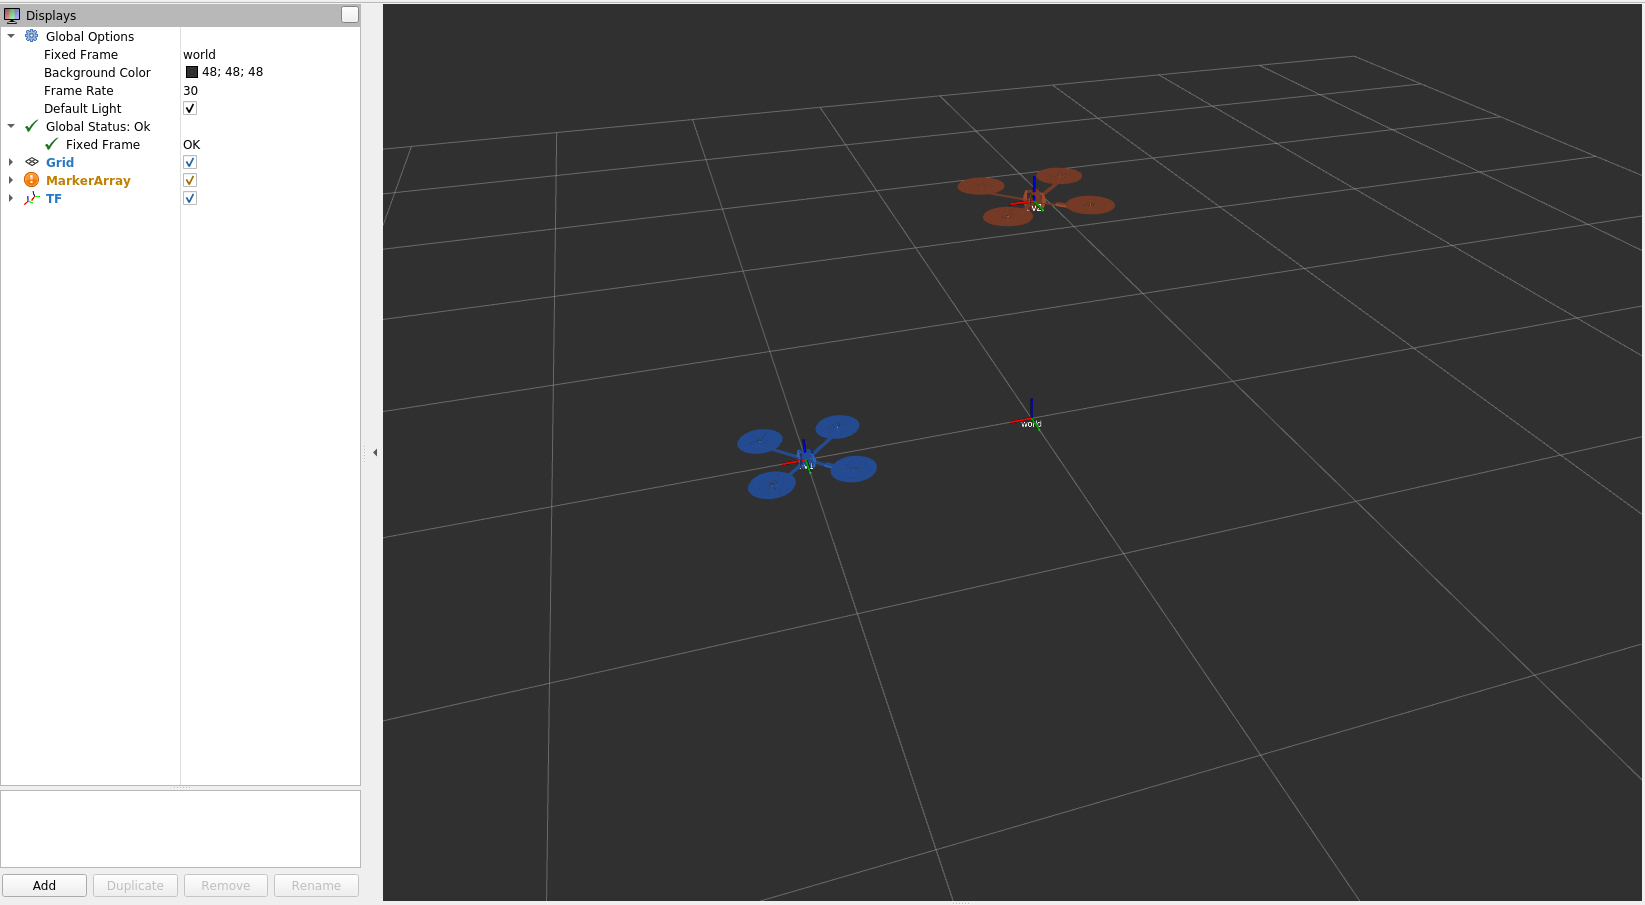
\includegraphics[width=\linewidth]{../results/screenshots/static_scene.png}
\caption{Static scenario, fixed frame \texttt{world}: AV1 (blue) at
$(1,0,0)$, AV2 (red) at $(0,0,1)$, with the TF axes of all frames.\protect\label{fig:static}}
\end{figure}

\begin{figure}[h]
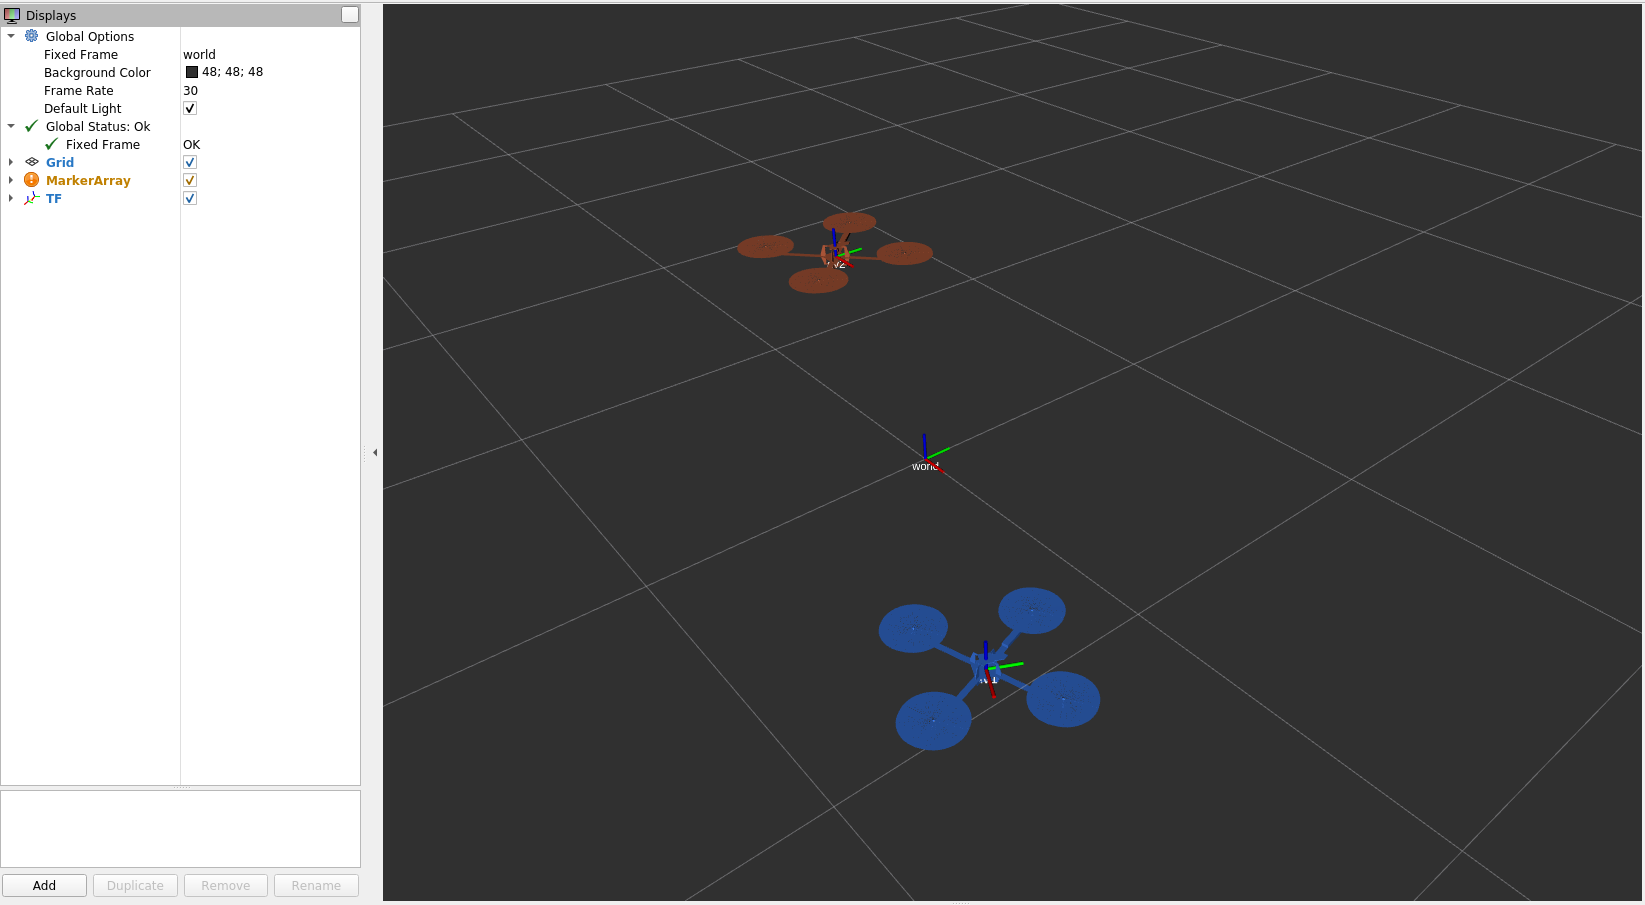
\includegraphics[width=\linewidth]{../results/screenshots/dynamic_world_a.png}
\caption{Moving scenario after Deliverable~2, before the trails were
implemented. The green $y$ axis of AV1 points along the circle.\protect\label{fig:dynamic}}
\end{figure}

\begin{marginfigure}
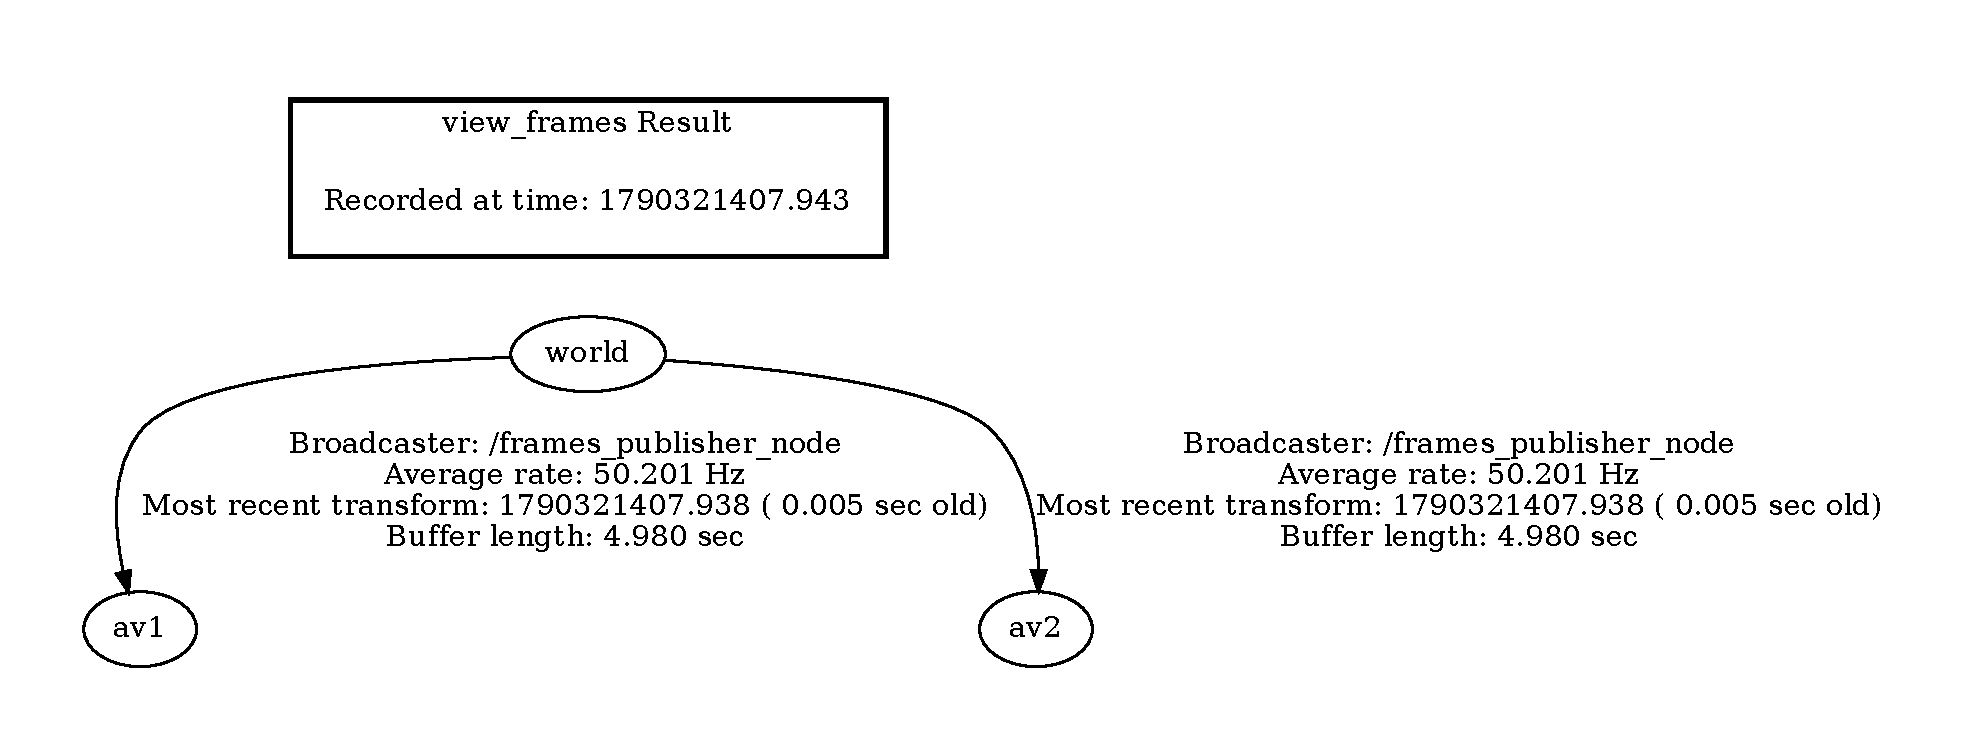
\includegraphics[width=\linewidth, trim=0 0 0 60, clip]{../results/screenshots/tf_tree_dynamic.pdf}
\caption{TF tree of the moving scenario (\texttt{rosrun tf view\_frames}).}
\label{fig:tftree}
\end{marginfigure}

\begin{evidence}
\cref{tab:pubsub,lst:manual,lst:nonstatic} and \cref{fig:markeroff} (four
questions); \cref{lst:frames} (implementation); \cref{fig:static,fig:dynamic}
(scenes); \cref{fig:tftree} and \texttt{dynamic\_nodes\_topics.txt}
(publisher and rates); \cref{tab:check} (orientation).
\end{evidence}

\gradeditem{sec:traj}{Trajectories and Reference Frames}{30}

\subsection{Querying the relative transform}

Each trail asks tf for the pose of \texttt{dest\_frame} in
\texttt{ref\_frame} (\cref{lst:lookup}).
\texttt{lookupTransform(target, source, time)} returns the transform that maps
coordinates from the source frame into the target frame, i.e.\
$T^{\mathrm{ref}}_{\mathrm{dest}}$; its translation is the origin of
\texttt{dest\_frame} expressed in \texttt{ref\_frame}, which is exactly the
point to append to the trail.
For the dashed trail the call is \texttt{lookupTransform("av1", "av2", ...)},
giving $\bm o_2^1$.
Swapping the arguments would return $T^2_1$, whose translation
$-R_z(t)\,\bm o_2^1$ traces a different curve.
\texttt{ros::Time(0)} requests the latest transform in the buffer; a failed
lookup raises \texttt{tf2::TransformException}, which the template catches, so
the sample is skipped instead of adding a zero point.
No lookup failed during the runs.
Two small changes support the display: the trail markers now carry an
identity orientation (RViz had warned about an uninitialised quaternion), and
the world trails keep 400 samples (\SI{8}{s} at \SI{50}{Hz}) instead of 300, so
that one full $2\pi$\,s period is visible.

\lstinputlisting[style=code, linerange={53-55}, firstnumber=53,
caption={Transform lookup in \texttt{TrajTrail::update()}.},
label=lst:lookup]{../two_drones_pkg/src/plots_publisher_node.cpp}

\subsection{Trajectories in RViz}

\Cref{fig:traj} shows the three trails.
With fixed frame \texttt{world}, AV1 draws the unit circle (blue), AV2 the
parabola arc in the $x$--$z$ plane (red, solid), and the dashed red curve is
AV2's path in \texttt{av1}, drawn in that moving frame.
With fixed frame \texttt{av1} the scene is seen from AV1: AV1 stays still,
the world axes spin about their $z$ axis, and the parabola rotates with them
(\cref{fig:traj}\,(b) and (c)).
The world origin stays at $(-1,0,0)$ in \texttt{av1} because
$R_z(t)^T(-\bm o_1^w) = (-1,0,0)^T$, and a circle turning about its own
centre looks unchanged, which is why the blue trail appears fixed as well.
The dashed trail is a closed curve on a slanted plane, the ellipse derived
in \cref{sec:math}.

\begin{figure*}[h]
\begin{tabular}{@{}c@{\hspace{4pt}}c@{\hspace{4pt}}c@{}}
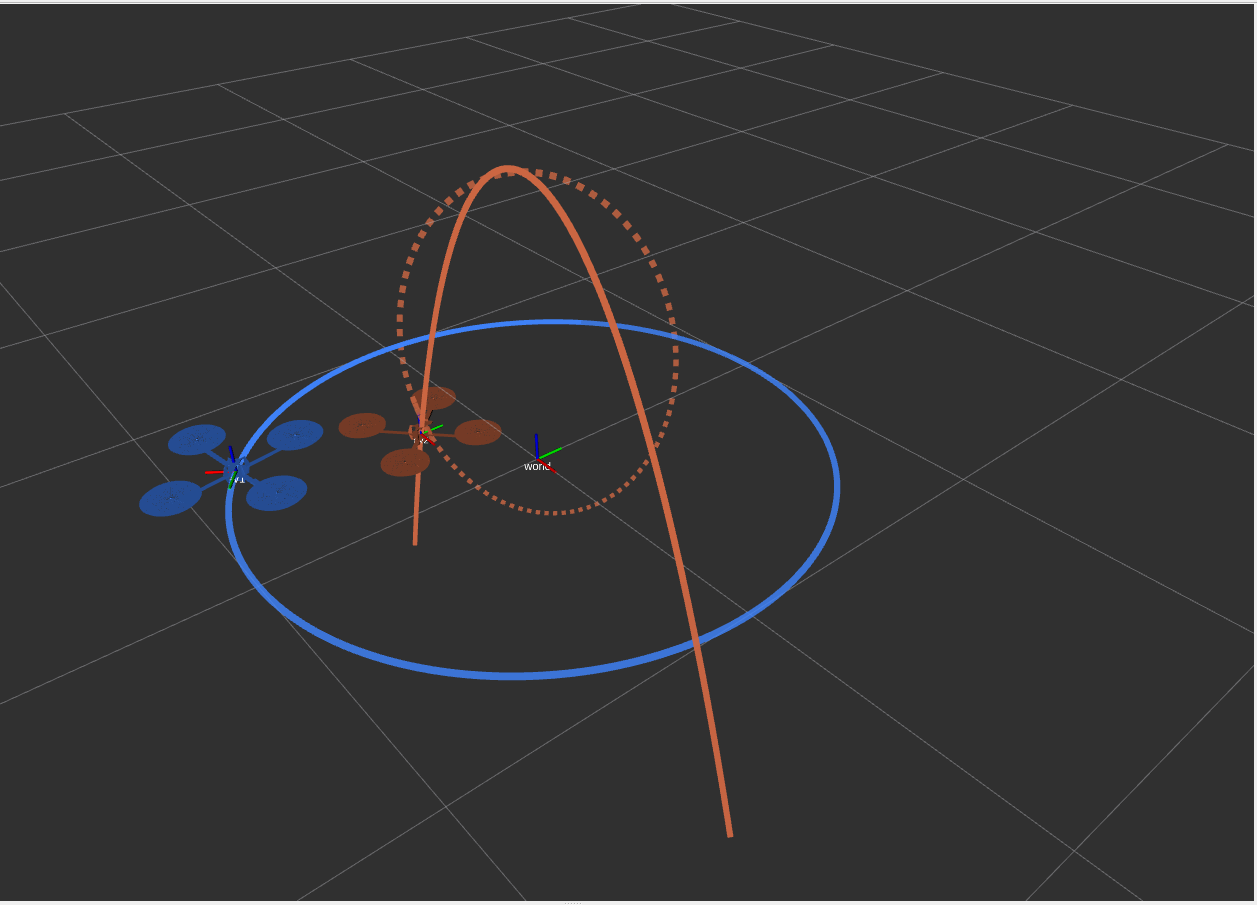
\includegraphics[width=0.325\linewidth]{figures/traj_fixed_world_view.png} &
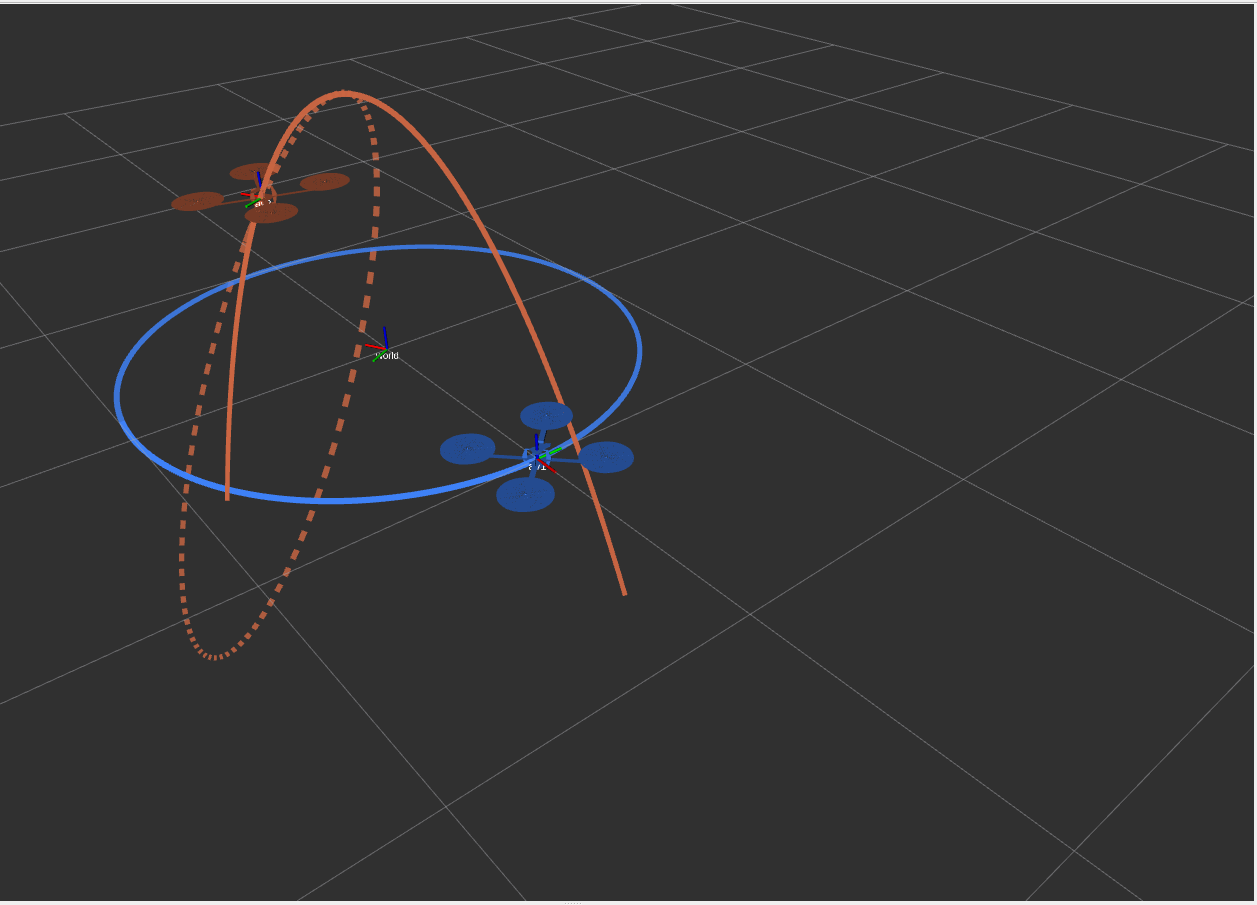
\includegraphics[width=0.325\linewidth]{figures/traj_fixed_av1_view.png} &
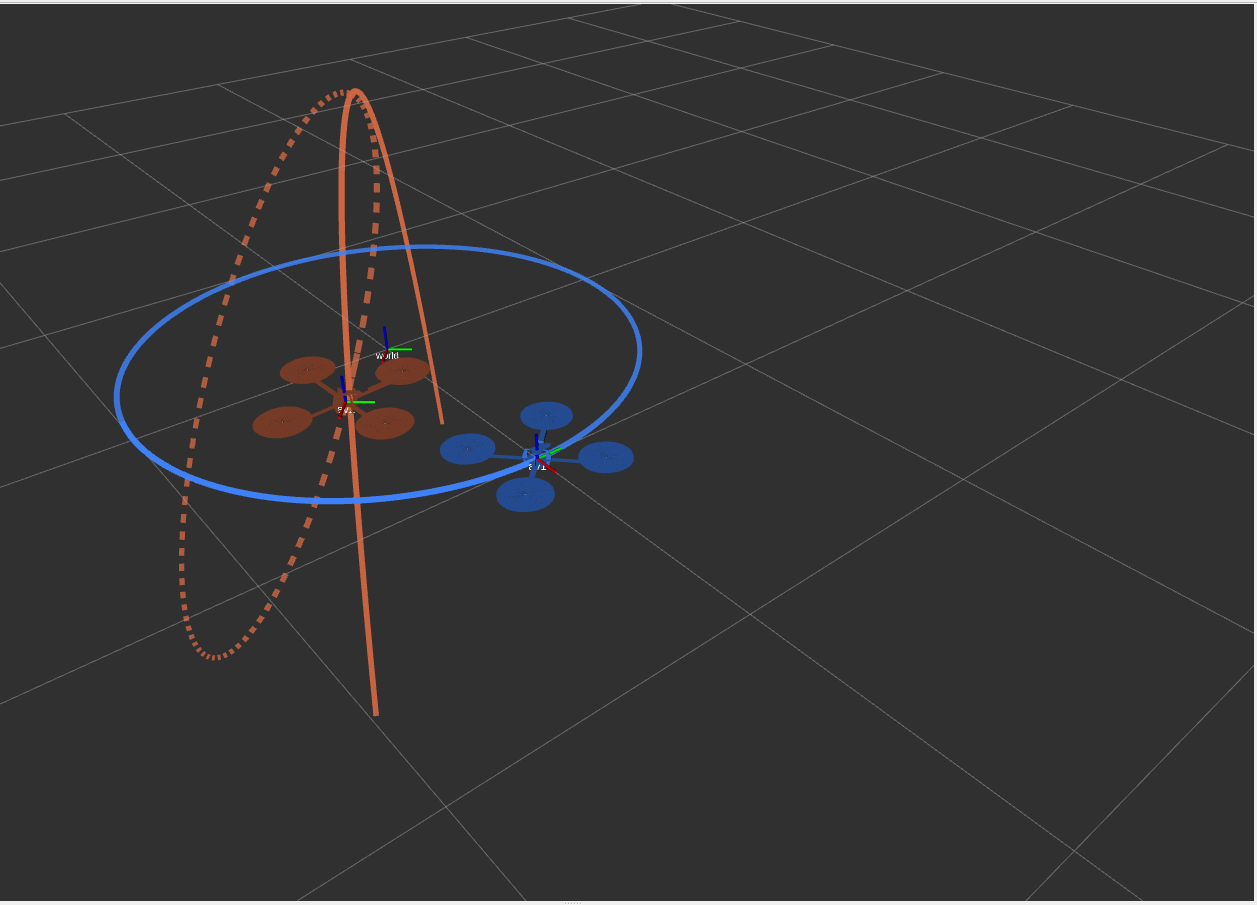
\includegraphics[width=0.325\linewidth]{figures/traj_fixed_av1_b_view.png} \\
\small (a) fixed frame \texttt{world} & \small (b) fixed frame \texttt{av1} &
\small (c) fixed frame \texttt{av1}, a few seconds later
\end{tabular}
\caption{Trails in RViz. Blue solid: AV1 in \texttt{world}; red solid: AV2 in
\texttt{world}; red dashed: AV2 in \texttt{av1}. From (b) to (c) AV1 stays in
place while the world-frame parabola rotates. 3D view cropped; the full RViz
windows, including the Fixed Frame setting, are in
\texttt{results/screenshots/traj\_fixed\_*.png}.\protect\label{fig:traj}}
\end{figure*}

\subsection{Numerical check}\label{sec:check}

To compare the tf data with the model, \texttt{scripts/check\_tf.py} looked
up \texttt{world}$\to$\texttt{av1}, \texttt{world}$\to$\texttt{av2} and
\texttt{av1}$\to$\texttt{av2} at a common stamp, 300 times over \SI{12}{s}.
The phase $t \bmod 2\pi = \operatorname{atan2}(y_1, x_1)$ of AV1 serves as the
time argument of the closed-form expressions of \cref{sec:math}.
It grows at \SI{1.000000}{rad/s} against the message stamps, so $t$ in the
publisher is indeed elapsed seconds.
\Cref{tab:check} lists the largest residuals; all are at double-precision
round-off, and the plane coordinates of the samples fill the ellipse of
\cref{fig:ellipse}.
This checks the geometry of the published and composed transforms; it does
not measure timing, which is covered by the rates in \cref{sec:drones}.

\begin{table}[h]
\small
\begin{tabularx}{\linewidth}{@{}X r@{}}
\toprule
Quantity & Max.\ $|\cdot|$ \\
\midrule
AV1: $x^2 + y^2 - 1$ & \num{2.2e-16} \\
AV1: yaw $-$ atan2$(y, x)$ [rad] & \num{4.4e-16} \\
AV1: $z$; roll/pitch part $\lVert(q_x, q_y)\rVert$ & 0 \\
AV2: $z - (1 - 2x^2)$ & \num{3.3e-16} \\
AV2: $y$; rotation angle & 0 \\
\texttt{av1}$\to$\texttt{av2} vs.\ $\bm o_2^1(t)$ of \cref{eq:o21} [m] & \num{6.1e-16} \\
Plane: $z - 2y - 1$ & \num{6.7e-16} \\
Plane frame: $z_p$ & \num{3.0e-16} \\
Plane frame: $x_p^2/(1/4) + y_p^2/(5/4) - 1$ & \num{1.8e-15} \\
\bottomrule
\end{tabularx}
\caption{Residuals of 300 tf samples against the model
(\texttt{results/logs/check\_tf\_summary.txt}). Measured ranges:
$x_p \in [-0.5000, 0.4999]$, $y_p \in [-1.1180, 1.1180]$.\protect\label{tab:check}}
\end{table}

\begin{marginfigure}
\begin{tikzpicture}
\begin{axis}[width=\linewidth, axis equal image, xmin=-0.7, xmax=0.7,
  ymin=-1.3, ymax=1.3, xlabel={$x_p$ [m]}, ylabel={$y_p$ [m]},
  tick label style={font=\scriptsize}, label style={font=\scriptsize},
  xtick={-0.5,0,0.5}, ytick={-1.118,0,1.118},
  yticklabels={$-\frac{\sqrt5}{2}$,0,$\frac{\sqrt5}{2}$}]
\addplot[domain=0:360, samples=120, black!50, thin] ({0.5*sin(x)}, {1.118034*cos(x)});
\addplot[only marks, mark=*, mark size=0.6pt, red!70!black]
  table[x=xp, y=yp, col sep=comma] {../results/logs/tf_samples.csv};
\end{axis}
\end{tikzpicture}
\caption{Relative position of AV2 in the plane frame: tf samples (dots) and
the ellipse of \cref{eq:ellipse} (grey).}
\label{fig:ellipse}
\end{marginfigure}

\begin{evidence}
\cref{lst:lookup} (implementation); \cref{fig:traj} (three trails in
both fixed frames); \cref{tab:check,fig:ellipse} and
\texttt{tf\_samples.csv} (numerical check).
\end{evidence}

\gradeditem{sec:math}{Mathematical Derivations}{10}

\paragraph{Notation.}
$T^a_b \in SE(3)$ is the pose of frame $b$ in frame $a$; it maps homogeneous
coordinates as $\tilde{\bm p}^a = T^a_b\,\tilde{\bm p}^b$, and
$T^a_c = T^a_b T^b_c$.
$\bm o_b^a$ is the origin of frame $b$ expressed in frame $a$.
Throughout, $c = \cos t$, $s = \sin t$, and
$R_z(t) = \left[\begin{smallmatrix} c & -s & 0\\ s & c & 0\\ 0 & 0 & 1\end{smallmatrix}\right]$.
From the problem statement,
\begin{equation*}
T^w_1 = \begin{bmatrix} c & -s & 0 & c\\ s & c & 0 & s\\ 0 & 0 & 1 & 0\\ 0 & 0 & 0 & 1 \end{bmatrix},
\qquad
T^w_2 = \begin{bmatrix} 1 & 0 & 0 & s\\ 0 & 1 & 0 & 0\\ 0 & 0 & 1 & \cos 2t\\ 0 & 0 & 0 & 1 \end{bmatrix}.
\end{equation*}

\paragraph{1. AV2 moves on an arc of a parabola.}
$\bm o_2^w = (s, 0, \cos 2t)^T$.
With $\cos 2t = 1 - 2\sin^2 t$ the coordinates satisfy
\begin{equation*}
y = 0, \qquad z = 1 - 2x^2, \qquad x = \sin t \in [-1, 1].
\end{equation*}
The path is therefore the part $-1 \le x \le 1$ of the parabola
$z = 1 - 2x^2$ in the $x$--$z$ plane, with vertex $(0, 0, 1)$ and end points
$(\pm 1, 0, -1)$; AV2 sweeps it back and forth with period $2\pi$.

\paragraph{2. Position of AV2 in AV1's frame.}
With $T^w_1 = \left[\begin{smallmatrix} R & \bm o_1^w\\ \bm 0^T & 1\end{smallmatrix}\right]$,
$R = R_z(t)$, the inverse is
$(T^w_1)^{-1} = \left[\begin{smallmatrix} R^T & -R^T\bm o_1^w\\ \bm 0^T & 1\end{smallmatrix}\right]$,
and $R^T \bm o_1^w = (c^2 + s^2,\, -sc + cs,\, 0)^T = (1, 0, 0)^T$. Hence
\begin{gather*}
(T^w_1)^{-1} = \begin{bmatrix} c & s & 0 & -1\\ -s & c & 0 & 0\\ 0 & 0 & 1 & 0\\ 0 & 0 & 0 & 1 \end{bmatrix},
\\
T^1_2 = (T^w_1)^{-1} T^w_2 = \begin{bmatrix} c & s & 0 & sc - 1\\ -s & c & 0 & -s^2\\ 0 & 0 & 1 & \cos 2t\\ 0 & 0 & 0 & 1 \end{bmatrix},
\end{gather*}
where the last column is $R^T\bm o_2^w - R^T\bm o_1^w = (cs, -s^2, \cos 2t)^T - (1, 0, 0)^T$.
Therefore
\begin{equation}\label{eq:o21}
\begin{aligned}
\bm o_2^1(t) &= \bigl(\sin t\cos t - 1,\; -\sin^2 t,\; \cos 2t\bigr)^T\\
&= \bigl(\tfrac12\sin 2t - 1,\; \tfrac12\cos 2t - \tfrac12,\; \cos 2t\bigr)^T .
\end{aligned}
\end{equation}
Simply subtracting the world positions, $\bm o_2^w - \bm o_1^w$, would give the
offset in world axes; the rotation $R^T$ is needed to express it in AV1's axes.
$\bm o_2^1$ has period $\pi$, whereas the full relative pose $T^1_2$ has
period $2\pi$ because of its rotation block.
Check values: $\bm o_2^1(0) = (-1, 0, 1)$, $\bm o_2^1(\pi/4) = (-\tfrac12, -\tfrac12, 0)$,
$\bm o_2^1(\pi/2) = (-1, -1, -1)$.

\paragraph{3. The relative path is planar.}
From \cref{eq:o21}, $y = -s^2$ and $z = 1 - 2s^2 = 1 + 2y$ for every $t$, so
all points lie in the plane
\begin{equation*}
\Pi:\; z - 2y - 1 = 0 \quad\text{(in AV1's frame)},\qquad
\bm n = \tfrac{1}{\sqrt5}(0, -2, 1)^T .
\end{equation*}

\paragraph{4. Coordinates in the plane.}
Take the origin $\bm p^1 = (-1, -\tfrac12, 0)^T$, which lies on $\Pi$
($0 + 1 - 1 = 0$), and the orthonormal axes
\begin{gather*}
\bm x_p = (1, 0, 0)^T, \qquad \bm y_p = \tfrac{1}{\sqrt5}(0, 1, 2)^T,\\
\bm z_p = \bm x_p \times \bm y_p = \tfrac{1}{\sqrt5}(0, -2, 1)^T = \bm n .
\end{gather*}
$\bm x_p$ and $\bm y_p$ are orthogonal to $\bm n$ and so lie in $\Pi$.
With $R^1_p = [\bm x_p\; \bm y_p\; \bm z_p]$,
\begin{gather*}
T^1_p = \begin{bmatrix} 1 & 0 & 0 & -1\\ 0 & \frac{1}{\sqrt5} & -\frac{2}{\sqrt5} & -\frac12\\ 0 & \frac{2}{\sqrt5} & \frac{1}{\sqrt5} & 0\\ 0 & 0 & 0 & 1 \end{bmatrix},
\\
(T^1_p)^{-1} = \begin{bmatrix} 1 & 0 & 0 & 1\\ 0 & \frac{1}{\sqrt5} & \frac{2}{\sqrt5} & \frac{1}{2\sqrt5}\\ 0 & -\frac{2}{\sqrt5} & \frac{1}{\sqrt5} & -\frac{1}{\sqrt5}\\ 0 & 0 & 0 & 1 \end{bmatrix}.
\end{gather*}
Using $\bm o_2^1 - \bm p^1 = (\tfrac12\sin 2t,\, \tfrac12\cos 2t,\, \cos 2t)^T$,
$\tilde{\bm o}_2^p = (T^1_p)^{-1}\,\tilde{\bm o}_2^1$ gives
\begin{align*}
x_p &= \tfrac12\sin 2t,\\
y_p &= \tfrac{1}{\sqrt5}\bigl(\tfrac12\cos 2t + 2\cos 2t\bigr) = \tfrac{\sqrt5}{2}\cos 2t,\\
z_p &= \tfrac{1}{\sqrt5}\bigl(-\cos 2t + \cos 2t\bigr) = 0 .
\end{align*}
$z_p$ vanishes as expected, and replacing $t$ by $-t$ or by $\pi/2 - t$
mirrors the curve in the $y_p$ or the $x_p$ axis, so both axes are axes of
symmetry.

\paragraph{5. The path is an ellipse.}
Eliminating $t$,
\begin{equation}\label{eq:ellipse}
\frac{x_p^2}{(1/2)^2} + \frac{y_p^2}{(\sqrt5/2)^2} = \sin^2 2t + \cos^2 2t = 1 ,
\end{equation}
an axis-aligned ellipse centred at $\bm p^1$ with semi-axes
$a = \tfrac12$ along $\bm x_p$ and $b = \tfrac{\sqrt5}{2} \approx 1.118$ along
$\bm y_p$, traversed once every $\pi$ seconds.
The tf samples reach $|x_p| = 0.5000$ and $|y_p| = 1.1180$ (\cref{tab:check}).

\begin{evidence}
Homogeneous transforms $T^w_1$, $T^w_2$, $(T^w_1)^{-1}$, $T^1_2$, $T^1_p$,
$(T^1_p)^{-1}$ with all intermediate steps; results confirmed against tf in
\cref{tab:check,fig:ellipse}.
\end{evidence}

\gradeditem{sec:quat}{Quaternion Properties}{10}

\paragraph{Conventions.}
A quaternion is $q = (q_1, q_2, q_3, q_4)^T = (\bm v, w)$ with vector part
$\bm v = (q_1, q_2, q_3)^T$ and scalar part $w = q_4$, and
$[\bm v]_\times$ is the skew-symmetric matrix with
$[\bm v]_\times \bm a = \bm v \times \bm a$.
The matrices of the handout\cite{vnav2023lab2} are, in block form,
\begin{equation*}
\Omega_1(q) = \begin{bmatrix} w I + [\bm v]_\times & \bm v\\ -\bm v^T & w \end{bmatrix},
\qquad
\Omega_2(q) = \begin{bmatrix} w I - [\bm v]_\times & \bm v\\ -\bm v^T & w \end{bmatrix}.
\end{equation*}
Applied to $y = (\bm v_y, w_y)$ and $x = (\bm v_x, w_x)$ they give
$\Omega_1(x)\,y = \Omega_2(y)\,x
= (w_x \bm v_y + w_y \bm v_x + \bm v_x \times \bm v_y,\; w_x w_y - \bm v_x^T\bm v_y)$,
which is the quaternion product $x \otimes y$ for \emph{all} $x, y \in \mathbb{R}^4$.
Two identities are used below:
$[\bm v]_\times^T = -[\bm v]_\times$ and
$[\bm v]_\times^2 = \bm v\bm v^T - \lVert\bm v\rVert^2 I$.
\marginnote{The slides print $\Omega_1$ with $(1,3)$ entry $-q_2$ and
$(2,3)$ entry $+q_1$; the handout has $+q_2$ and $-q_1$. The slide version
is not orthogonal (a random unit $q$ gives
$\max|\Omega_1^T\Omega_1 - I| = 0.999$) and is taken as a typo.
\texttt{scripts/quaternion\_check.py} also checks all three properties
numerically; this is a sanity check, not a proof.}

\paragraph{1. Orthogonality.}
Write $\Omega_i(q) = \left[\begin{smallmatrix} A & \bm v\\ -\bm v^T & w\end{smallmatrix}\right]$
with $A = wI + \epsilon[\bm v]_\times$, $\epsilon = +1$ for $\Omega_1$ and
$-1$ for $\Omega_2$. Then
\begin{equation*}
\Omega_i^T\Omega_i =
\begin{bmatrix} A^T A + \bm v\bm v^T & A^T\bm v - w\bm v\\ \bm v^T A - w\bm v^T & \bm v^T\bm v + w^2 \end{bmatrix}.
\end{equation*}
Since $A^T = wI - \epsilon[\bm v]_\times$ and $\epsilon^2 = 1$,
$A^T A = w^2 I - [\bm v]_\times^2 = (w^2 + \lVert\bm v\rVert^2) I - \bm v\bm v^T$,
so the top-left block is $\lVert q\rVert^2 I$.
The off-diagonal blocks vanish because
$A^T\bm v - w\bm v = -\epsilon\,\bm v \times \bm v = \bm 0$,
and the bottom-right entry is $\lVert q\rVert^2$.
Hence $\Omega_i(q)^T\Omega_i(q) = \lVert q\rVert^2 I_4 = I_4$ for a unit
quaternion; a square matrix whose transpose is a left inverse also has it as a
right inverse, so $\Omega_i(q)\Omega_i(q)^T = I_4$ as well.

\emph{Intuition.} For unit $q$ and every unit $x$, $q \otimes x$ and
$x \otimes q$ are again unit quaternions, i.e.\
$\lVert\Omega_1(q)x\rVert = \lVert\Omega_2(q)x\rVert = 1$.
By linearity both maps preserve the length of every vector in $\mathbb{R}^4$,
and a linear map that preserves lengths is orthogonal.

\paragraph{2. Mapping $q$ to the identity.}
The last column of both matrices is $q$, so
$\Omega_i(q)\,\bm e_4 = q$ with $\bm e_4 = (0, 0, 0, 1)^T$, the identity
rotation ($q \otimes 1 = 1 \otimes q = q$).
Multiplying by $\Omega_i(q)^T$ and using part~1,
\begin{equation*}
\Omega_i(q)^T q = \Omega_i(q)^T\Omega_i(q)\,\bm e_4 = \bm e_4 = (0, 0, 0, 1)^T .
\end{equation*}
Equivalently, $\Omega_1(q)^T = \Omega_1(q^*)$ with the conjugate
$q^* = (-\bm v, w)$, so the statement reads $q^* \otimes q = 1$.

\paragraph{3. Commutation.}
For arbitrary $x, y, z \in \mathbb{R}^4$, using $\Omega_1(a)b = a \otimes b$,
$\Omega_2(b)a = a \otimes b$ and the associativity of quaternion
multiplication,
\begin{equation*}
\Omega_1(x)\Omega_2(y)\,z = x \otimes (z \otimes y)
= (x \otimes z) \otimes y = \Omega_2(y)\Omega_1(x)\,z .
\end{equation*}
Since this holds for every $z$, $\Omega_1(x)\Omega_2(y) = \Omega_2(y)\Omega_1(x)$.
For the second identity note that
$\Omega_2(y)^T = \left[\begin{smallmatrix} w_y I + [\bm v_y]_\times & -\bm v_y\\ \bm v_y^T & w_y\end{smallmatrix}\right] = \Omega_2(y^*)$,
because $[-\bm v_y]_\times = -[\bm v_y]_\times$.
Applying the first identity to $x$ and $y^*$ gives
$\Omega_1(x)\Omega_2(y)^T = \Omega_2(y)^T\Omega_1(x)$.
Neither argument needs $x$ or $y$ to be unit quaternions.

\begin{evidence}
Proofs of the three properties with block matrices; note on the sign
difference in the slides; numerical sanity check in
\texttt{results/logs/quaternion\_check.txt} (largest deviation
\num{1.8e-15} over 1000 random cases).
\end{evidence}

\section{Discussion}

\paragraph{Problems met.}
\begin{itemize}
\item \emph{Expired ROS key.} Older guides import the ROS key with
\texttt{apt-key}; that key expired in June~2025. The \texttt{ros-apt-source}
package installs the current key and source.
\item \emph{Network in WSL.} Windows uses a local proxy, which WSL~2 cannot
reach in its default NAT mode; \texttt{raw.githubusercontent.com}, needed by
\texttt{rosdep}, timed out. Switching WSL to mirrored networking with
\texttt{autoProxy} passes the Windows proxy through.
\item \emph{Invisible windows.} When WSL was started from the SSH session,
WSLg created its display client in that non-interactive Windows session and
the turtlesim window stayed unmapped. Starting WSL from the desktop first
fixed it.
\item \emph{Display manager.} \texttt{desktop-full} pulls in \texttt{gdm3},
which tried to start under systemd inside WSL; it was disabled.
\item \emph{Missing meshes.} RViz drew the grid and TF axes but not the drone
meshes with the WSLg D3D12 OpenGL driver (OpenGL~3.1 on an RTX~4070~SUPER).
Software rendering (\texttt{LIBGL\_ALWAYS\_SOFTWARE=1}) draws them correctly
at \SI{30}{fps}, but RViz then uses about 1.7 CPU cores. When the plotting
timer is delayed, consecutive trail samples are far apart and the line strip
shows a short chord; it leaves the trail once the gap drops out of the
buffer.
\item \emph{Template and slides.} The member-order defect in
\texttt{plots\_publisher\_node} and the sign typo in the slides' $\Omega_1$
were found and handled as described above.
\end{itemize}

\paragraph{Reflections.}
The lab turns abstract transform notation into things that can be seen.
Three details decided whether the result was right: the direction of a
transform (\texttt{lookupTransform(ref, dest)} gives $T^{\mathrm{ref}}_{\mathrm{dest}}$,
and the swapped call draws a different curve), the orientation of AV1 (with
yaw $t + \pi/2$ the relative path turns by $90^\circ$ about $z_1$ and lies on
$z = 1 + 2x$ instead, so the plane and the hinted origin no longer fit), and the need to rotate, not only
subtract, when changing frames.
Checking the ROS output against the closed-form result made each of these
testable instead of a matter of how the RViz picture looks.

\section{Conclusions}
ROS Noetic was installed and tested with turtlesim.
The two-drone scenario was analysed through its nodes, topics and launch
file, the drone poses were published with \texttt{tf2}, and the relative
transform was looked up to draw the three trails.
The relative path of AV2 in AV1's frame is an ellipse on the plane
$z - 2y = 1$ with semi-axes $\tfrac12$ and $\tfrac{\sqrt5}{2}$, derived with
homogeneous transforms and matched by the tf data to round-off level.
The quaternion multiplication matrices were shown to be orthogonal, to map
$q$ to the identity, and to commute.

\bibliography{refs}
\bibliographystyle{plainnat}

\end{document}
